\section{Pregunta N$^{\circ}$5\qquad Andre Gilmer Santos Felix}

\begin{frame}
    \begin{enumerate}\setcounter{enumi}{4}
        \item

              Determine si la función
              \begin{math}
                  S\left(x\right)=
                  \begin{cases}
                      1+
                      x-
                      x^{3},                   & 0 \leq x<1      \\
                      1-
                      2\left(x-1\right)-
                      3{\left(x-1\right)}^{2}+
                      4{\left(x-1\right)}^{3}, & 1 \leq x<2      \\
                      4\left(x-2\right)+
                      9{\left(x-2\right)}^{2}-
                      3{\left(x-2\right)}^{3}, & 2 \leq x \leq 3
                  \end{cases}
              \end{math}
              es el \alert{spline cúbico natural} que interpola en
              los puntos $\left(0,1\right)$, $\left(1,1\right)$,
              $\left(2,0\right)$ y $\left(3,10\right)$.
    \end{enumerate}

    \begin{solution}
        Chequeremos las tres propiedades de la función spline cúbico natural.

        \begin{description}
            \item[Propiedad 1]

                Existen $n=4$ puntos de datos.
                Debemos chequear
                \begin{align*}
                     & S_{1}\left(0\right)=1\quad\text { y }\quad S_{1}\left(1\right)=1.  \\
                     & S_{2}\left(1\right)=1\quad\text { y }\quad S_{2}\left(2\right)=0.  \\
                     & S_{3}\left(2\right)=0\quad\text { y }\quad S_{3}\left(3\right)=10.
                \end{align*}
                % These follow easily from the defining equations (3.18).

            \item[Propiedad 2]

                Las primeras derivadas de las funciones spline son

                \begin{align*}
                     & S_1^{\prime}\left(x\right)=
                    -\frac{13}{8}+\frac{15}{8}(x-1)^2.                 \\
                     & S_2^{\prime}\left(x\right)=
                    \frac{1}{4}+\frac{15}{4}(x-2)-\frac{15}{8}(x-2)^2. \\
                     & S_3^{\prime}\left(x\right)=
                    \frac{1}{4}-\frac{15}{4}(x-4)+\frac{15}{8}(x-4)^2.
                \end{align*}

                We must check $S_1^{\prime}(2)=S_2^{\prime}(2)$ and
                $S_2^{\prime}(4)=S_3^{\prime}(4)$.
                The first is
                \begin{math}
                    -\frac{13}{8}+
                    \frac{15}{8}=
                    \frac{1}{4}
                \end{math}
                and the second is
                \begin{math}
                    \frac{1}{4}+
                    \frac{15}{4}(4-2)-
                    \frac{15}{8}(4-2)^2=
                    \frac{1}{4},
                \end{math}
                both of which check out.
        \end{description}
        % \begin{math}
        %     \left[
        %         0,3
        %         \right]
        % \end{math}.

        % \begin{math}
        %     \forall j\in\left\{0,\dotsc,n-1\right\}:
        %     S_{j}\left(x_{j}\right)=
        %     f\left(x_{j}\right),
        %     S_{j+1}\left(x_{j+1}\right)=
        %     f\left(x_{j+1}\right),
        % \end{math}
    \end{solution}
\end{frame}

\begin{frame}
    \begin{solution}
        \begin{description}
            \item[Propiedad 3]

                The second derivatives are

                \begin{align*}
                     & S_1^{\prime\prime}\left(x\right)=\frac{15}{4}(x-1)                 \\
                     & S_2^{\prime\prime}\left(x\right)=\frac{15}{4}-\frac{15}{4}(x-2)    \\
                     & S_3^{\prime\prime}\left(x\right)=-\frac{15}{4}+\frac{15}{4}(x-4) .
                \end{align*}
                We must check $S_1^{\prime \prime}(2)=S_2^{\prime \prime}(2)$ and $S_2^{\prime \prime}(4)=S_3^{\prime \prime}(4)$, both of which are true.
        \end{description}
        Therefore, (3.18) is a cubic spline.
    \end{solution}
\end{frame}

\begin{frame}
    \begin{solution}
        \begin{figure}[ht!]
            \centering
            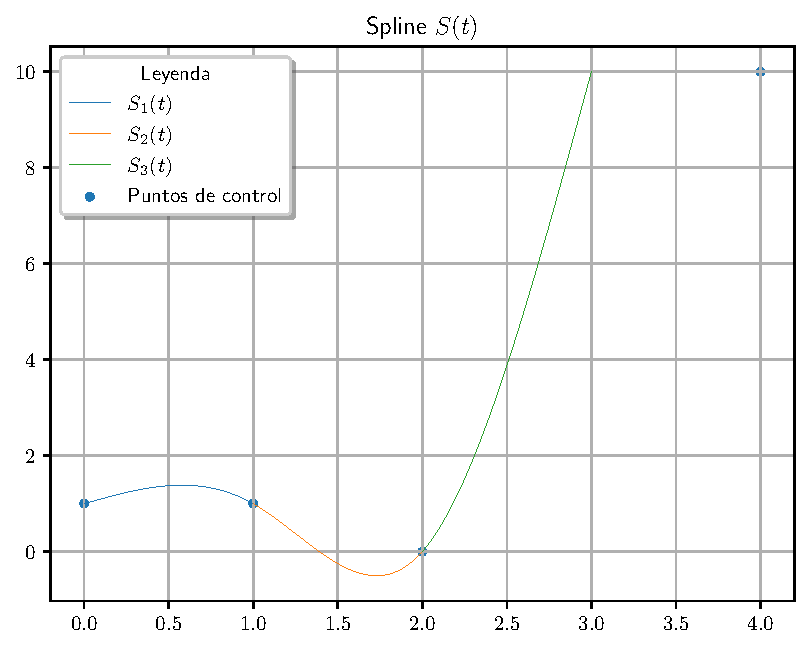
\includegraphics[width=.72\paperwidth]{p5}
        \end{figure}
    \end{solution}
\end{frame}